%
%	z.B. Text des zweiten Autors
%

\section{Weitere Kommandos}

\subsection{Mathematische Formeln}

Mathematische Formeln werden mittels \verb|\(...\)|
in den Fließtext eingebaut
--- zum Beispiel \( E=mc^2 \) und:
sei \(V\) ein Vektorraum über \(\mathbb{R}\)
und \(\mathcal{M}\) eine Indexmenge
---
oder aber mittels \verb|\[...\]|
abgesetzt und zentriert dargestellt:
	\[
	\pmb{x} = \sqrt[3]{\frac{a^2-b^2}{a^2+b^2}}
		~~~~~ \text{versus} ~~~~~
	\boldsymbol{x} = \sqrt[3]{\frac{a^2-b^2}{a^2+b^2}}
	\]


\subsection{Silbentrennung}
Vertrauen Sie bitte nie einer automatischen Silbentrennung (auch nicht der von Microsoft Word \& Co.). In folgendem Test-Absatz ist das Wort "`Spracherkennung"' falsch getrennt.

Testzeile Testzeile Testzeile Testzeile Testzeile Testzeile Testzeile Testzeile Te Spracherkennung.

Sie können LaTeX die richtige Trennung mit \verb|\hyphenation{...}| mitteilen. Man tut das üblicherweise noch vor \verb|\begin{document}|.

\hyphenation{Sprach-er-ken-nung}	% hier jetzt zu Demonstrationszwecken im Text
Testzeile Testzeile Testzeile Testzeile Testzeile Testzeile Testzeile Testzeile Te Spracherkennung.


\subsection{Literaturzitate}
\label{sec:literaturzitate}

Im Lehrbuch \cite{Schukat-Talamazzini1995}
finden sich Hinweise auf einschlägige Verfahren der automatischen Spracherkennung.

Das Literaturverwaltungsprogramm JabRef \cite{Kopp2018} ist für viele Plattformen verfügbar und unterstützt bei der Literaturrecherche. Es ist prädestiniert dazu, mit {\LaTeX} in Kombination mit {Bib\TeX} zusammenzuarbeiten.

Über die Literaturrecherche haben Sie Zugriff auf das Buch "`Das Textverarbeitungssystem LaTeX"' \cite{Oechsner2015}. Hierzu können Sie auch direkt den DOI-Link im Literaturverzeichnis anklicken.

\subsection{Einbinden von Bildern}

Sie können mit der Anweisung \verb|\includegraphics{datei}| eine Grafikdatei einbinden. Diese kann im PDF-, JPG- oder PNG-Format vorliegen. Grafiken werden üblicherweise in die float-Umgebung \verb|figure| gekapselt. Der Assistent in TeXstudio \cite{vanderZander2018} tut dies automatisch, wenn das Verhalten nicht explizit abgeschaltet wird. Jede eingebundene Grafik muss vom Text aus referenziert werden. Die textuelle Referenz hat \textit{vor} der Grafik zu erfolgen. Ein eingebundenes PDF ist in \autoref{fig:AufbauMustererkennungssystem} zu sehen.

\begin{figure}[tb]
\centering
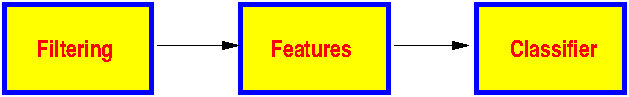
\includegraphics [height=20mm] {images/bildchen}
\caption {Aufbau eines Mustererkennungssystems}
\label{fig:AufbauMustererkennungssystem}
\end{figure}

Auch andere Grafikformate werden unterstützt. Verwenden Sie den Assistenten in TeXstudio, um komfortabel Grafiken einzufügen. Siehe dazu \autoref{fig:GrafikEinfuegen}. Die Grafiken finden sich nicht notwendigerweise direkt am Einfüge-Ort. Das Textsatzsystem richtet es so ein, dass es gut aussieht.

\begin{figure}
\centering
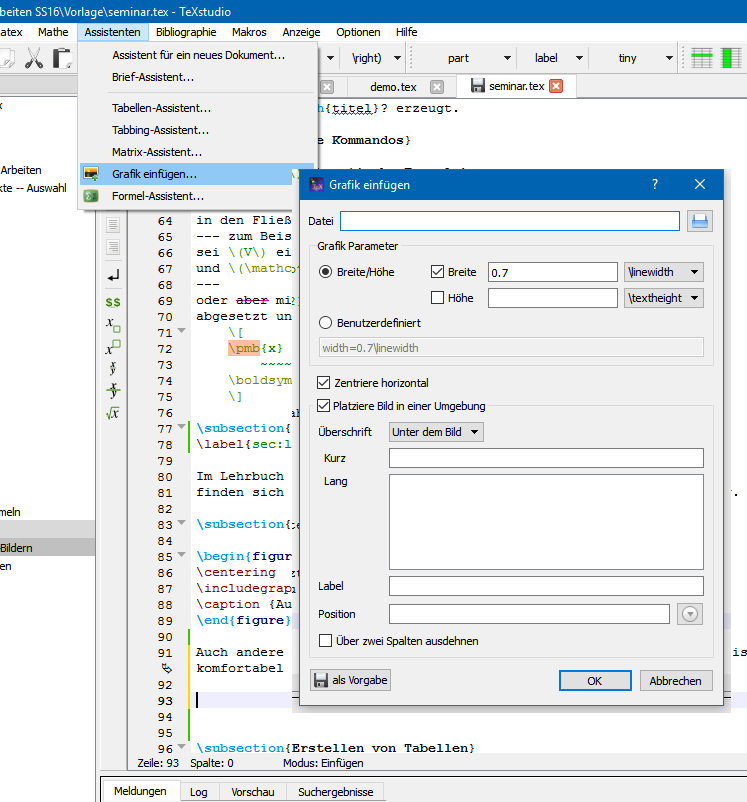
\includegraphics[width=0.7\linewidth]{images/GrafikEinfuegen}
\caption{Verwendung des Assistenten, um eine Grafik einzufügen.}
\label{fig:GrafikEinfuegen}
\end{figure}

\blindtext

\blindtext

\blindtext
\blindtext

\subsection{Querverweise}\label{sec:querverweise}
Verwenden Sie unter TeXstudio die rechte Maustaste in der Strukturübersicht, um für einen Abschnitt ein Label zu erzeugen, auf das Sie Bezug nehmen können (siehe \autoref{fig:LabelErzeugen}).

\begin{figure}
\centering
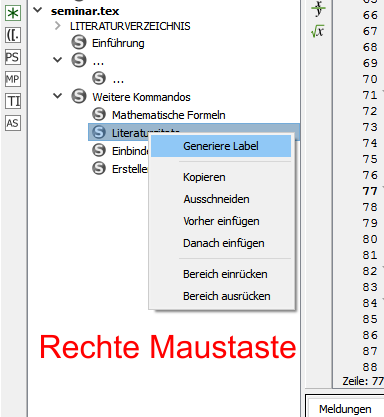
\includegraphics[width=0.4\linewidth]{images/LabelErzeugen}
\caption{Automatische Erzeugung eines Labels für Querverweise}
\label{fig:LabelErzeugen}
\end{figure}

Es wird ein Eintrag \verb|\label{key}| erzeugt, auf den man beispielsweise mit
\verb|\autoref{key}| verweisen kann. Verwendet man \verb|\autoref|, wird der Typ des Objekts
(z.\,B. Abbildung, Tabelle, etc.) mit ausgegeben. Verwendet man nur \verb|\ref|,
so wird nur die Nummerierung des Objekts ausgegeben.

\subsection{Erstellen von Tabellen}

Das Volk hat gesprochen. Siehe \autoref{tab:tabular}. Auch hier kommt ein float zum Einsatz, jedoch mit dem Positionierungs-Hinweis \verb|[h]|. Jedes float sollte mit einem Label versehen werden, und es sollte im Text darauf verwiesen werden, da sich die Position ändern kann.

\begin{table}[h]
\centering
\begin{tabular} {|llc||r|}
	\hline
	Name & Rang & Fraktion & Stimmenanteil \\
	\hline
	Mobutu & General & CDU & 57\% \\
	Tsvangirai & Oberst & CSU & 63\% \\
	\hline
\end{tabular}
\caption {Bundestagswahl in Simbabwe}
\label{tab:tabular}
\end{table}

\autoref{tab:booktab} verwendet keine vertikalen Linien und entspricht dem üblicherweise in Büchern verwenden Stil. Derartige Tabellen sind deutlich ansehnlicher.

\begin{table}[h]
\centering
\begin{tabular} {llcr}
	\toprule
	Name & Rang & Fraktion & Stimmenanteil \\
	\midrule
	Mobutu & General & CDU & 57\% \\
	Tsvangirai & Oberst & CSU & 63\% \\
	\bottomrule
\end{tabular}
\caption {Bundestagswahl in Simbabwe}
\label{tab:booktab}
\end{table}

\subsection{Listen und Aufzählungen}

Listen und Aufzählungen werden in einer Umgebung angelegt (umschlossen von \verb|begin| und \verb|end|.). \verb|\begin{itemize}| leitet eine Liste ein und \verb|\begin{enumerate}| eine Aufzählung. Die Einträge werden jeweils mit \verb|\item| begonnen. Folgend zwei Beispiele.

Itemize:
\begin{itemize}
\item Test
\item Test
\item Test
\end{itemize}

Enumerate:
\begin{enumerate}
\item Test
\item Test
\item Test
\end{enumerate}